\chapter{Beschleunigungssensor}
\label{ch:Beschleunigungssensor}
Um den Energieverbrauch der WLAN-basierten Lösungen zu senken wird in diesem Kapitel die Einbindung eines Beschleunigungssensors diskutiert. \\
Im Tunnel Rastatt, in dem auch die Versuche stattfanden, arbeiten die Bauarbeiter in zwei Schichten zu je zwölf Stunden. 
Nach zehn Tagen Schicht hat ein Arbeiter fünf Tage frei, jeder Arbeiter arbeitet also genau ein Drittel der Gesamtzeit. \\
Die mobile Einheit behält jedoch derzeit seinen Senderythmus bei, angesichts des hohen Stromverbrauchs beim Senden ist dies ineffizient.
Ein Beschleunigungssensor soll bestimmen, wann die mobile Einheit in Bewegung ist. 
Dadurch wird sie nicht mehr senden, wenn sie nicht getragen wird.

\section{LIS3DH}
Der LIS3DH ist ein drei Achsen Beschleunigungssensor von ST Microelectronics \cite{st2015lis}.
Er zeichnet sich durch einen ultra-low-power Modus und einen Pin für externe Unterbrechung (Interrupt) aus.
Der Beschleunigungssensor bietet ein $I^2C$ und ein SPI Interface um ihn zu konfigurieren.
Der LIS3DH benötigt bei einer Frequenz von einem Herz nur 2 Mikroamper (0,002 mA).\\
Leider konnte bei einem Herz der Interrupt durch Laufbewegungen nicht sicher ausgelöst werden, die Frequenz wurde deshalb auf zehn Herz erhöht.
Für eine Frequenz von zehn Herz im ultra-low-power Modus listet das Datenblatt einen Verbrauch von 3 Mikroamper.
Abbildung \ref{fig:lis3dh} zeigt eine Platine mit integriertem LIS3DH.

\begin{figure}[h]
  \centering
	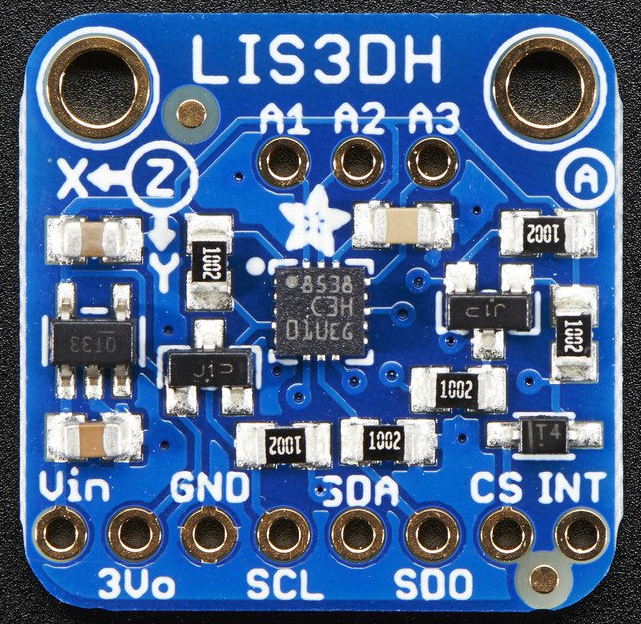
\includegraphics[width=0.5\textwidth]{images/lis3dhada.png}
  \caption{LIS3DH integriert auf einer Platine für die Entwicklung. Bild von Adafruit Industries.}
  \label{fig:lis3dh}
\end{figure}

\section{Abschaltautomatik}
\label{ch:Beschleunigungssensor:sec:Abschaltautomatik}
Der ESP8266 besitzt einen Enable Pin, ist dieser mit der Versorungsspannung verbunden werden die internen Spannungregler aktiviert und der ESP8266 mit Strom versorgt.
Die eigentliche Stromversorgung bezieht er dabei jedoch aus dem Vcc Pin.
Der ESP8266 soll durch den LIS3DH angeschaltet werden, der ESP8266 darf die Stromversorgung bei Bedarf trennen, sie kann danach wieder vom LIS3DH wieder aktiviert werden. \\
Um dieses Verhalten zu erreichen wird ein Latch eingesetzt \cite{texas2003latch}.
Es handelt sich dabei um einen digitalen Schalter mit einem SET Eingang (An), einem RESET Eingang (Aus) und einem Ausgang.
Der Ausgang wird mit dem Enable Pin verbunden, ist er aktiv, wird der ESP8266 aktiv.
Der SET Eingang wird mit dem interrupt Pin des LIS3DH verbunden, er kann damit den den Ausgang aktivieren.
Der RESET Eingang wird mit dem ESP8266 verbunden. 
Es wurde Pin 16 ausgewählt, da dieser für das Aufwecken aus dem Tiefschlaf zuständig ist. 
Stattdessen soll er nun die Stromversorgung abschalten und durch die zuvor im \texttt{deep\_sleep} verbrachte Zeit das Sendeintervall abwarten.\\
Da das Aufwecken mit Pin 16 durch das Verbinden des Pins mit der Masse funktioniert, kann damit nicht direkt der RESET Eingang des Latches betrieben werden.
Stattdessen wird das Ergebnis von Pin 16 mit der Versorgungsspannung über ein XOR Gatter verschaltet und mit dem RESET Eingang verbunden \cite{texas2014xor}.
Abbildung \ref{fig:schematics} zeigt das Schema der Verbindung von ESP8266 und LISD3H.

\begin{figure}[h]
  \centering
	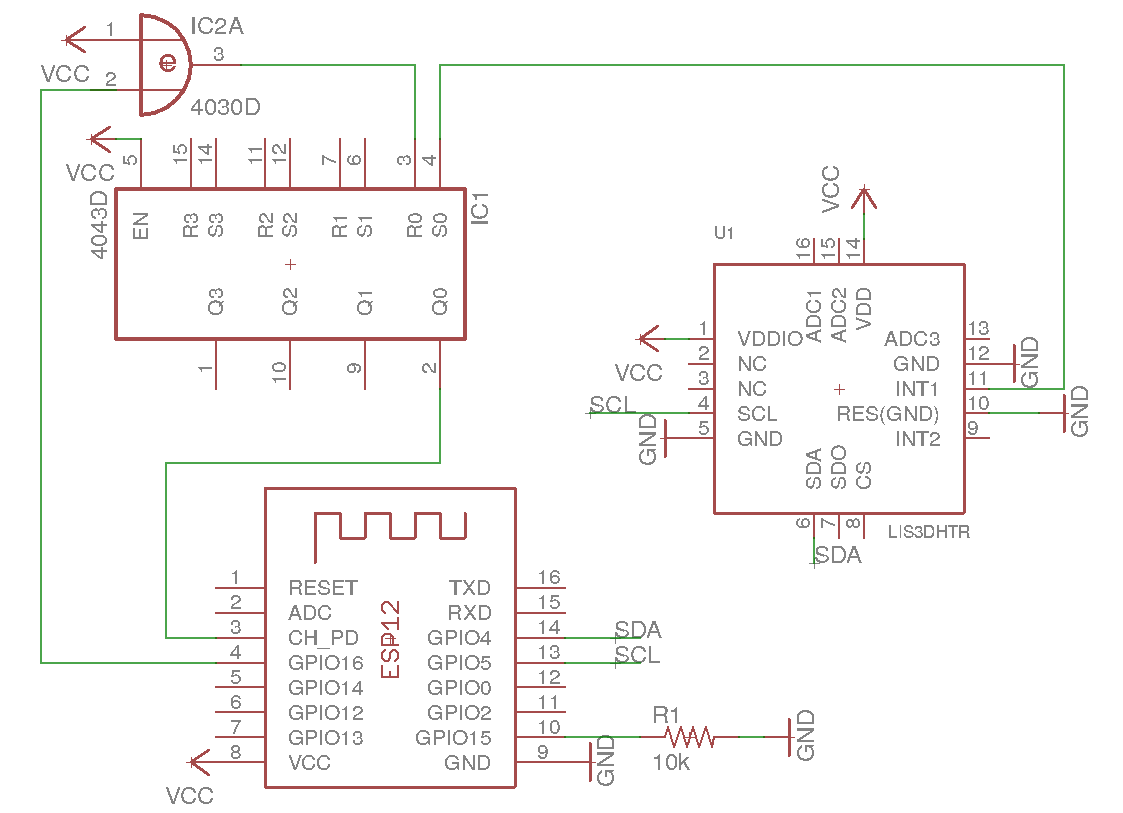
\includegraphics[width=\textwidth]{images/schematics.png}
  \caption{Schema der Verbindung von ESP8266 und LIS3DH.}
  \label{fig:schematics}
\end{figure}

\section{Bewertung}
Der Verbrauch des Beschleunigungssensors ersetzt lediglich den Verbrauch des Mikrocontrollers, die anderen Komponenten bleiben davon unberührt.
Zu den 3 Mikroamper Verbrauch addiert sich deshalb der Verbrauch des Spannungswandlers (55 Mikroamper) und des Lithium-Polymer-Ladeschaltkreises (bis zu 100 Mirkoamper).
Hinzu kommen bis zu 1 Mikroamper für das Latch und 10 Mikroamper für das XOR Gatter.\\
Die Integration des Beschleunigungssensor kann also den Verbrauch des ESP8266 außerhalb der Arbeitszeiten durch einen Verbrauch von 14 Mikroamper ersetzen, die bis zu 166 Mikroamper Verbrauch der umliegenden Komponenten bleibt jedoch vorhanden.
Die Laufzeit für eine nicht bewegte mobilen Einheit mit ESP8266 beträgt dann mindestens $1400mAh / 0,18mA = 7777,77h$, dies entspricht ca. 324 Tagen.\\
Für die mobile Einheit mit dem nRF52 Bluetooth-Chip macht die Integration des Beschleunigungssensors keinen Sinn, da der mittlere Verbrauch dieses Mikrocontrollers nur ca. 2 Mikroamper über dem des Beschleunigungssensors liegt.

